\documentclass[11pt,a4paper]{scrartcl}

\usepackage{fullpage}

%\usepackage[ngerman]{babel}
\usepackage[utf8]{inputenc}
\usepackage{graphicx}

\usepackage{amsmath}
\usepackage{amsthm}
\usepackage{mathtools}

\usepackage{listings}

%%%%% COMMANDS

\newcommand{\FT}{\mathcal{F}}
\newcommand{\T}{\mathrm{T}}
\newcommand{\IFT}{\mathcal{F}^{-1}}
\newcommand{\conv}{\ast}
\newcommand{\defined}{\coloneqq}

\newtheorem*{theorem}{Theorem}

\renewcommand{\thesubsection}{\alph{subsection})}

\begin{document}

\title{Artificial Intelligence Excercise Sheet 1}
\author{Markus Döring, 3153320}
\maketitle

\section{PEAS}
\subsection{Soccer}
\begin{description}
 \item[Performance Measure] The final result of the game (win or lose), perhaps some egoistic goals (not getting injured, scoring many goals)
 \item[Environment] The field, the ball, other players, lighting, spectators
 \item[Actuators] Muscles, in general (legs, chest, head, \ldots)
 \item[Sensors] The human senses (eyes, ears, \ldots)
\end{description}
\subsection{Titan Rover}
\begin{description}
 \item[Performance Measure] Robot performs experiments successfully, without getting lost
 \item[Environment] A whole world
 \item[Actuators] Wheels, robot arm, some kind of rocket engine
 \item[Sensors] Camera (normal light, infrared), temperature sensors, radar
\end{description}
\subsection{Bidder}
\begin{description}
 \item[Performance Measure] The final price of the object, and whether he actually gets it
 \item[Environment] Auctionator, other bidders, bank account
 \item[Actuators] Arm (for raising)
 \item[Sensors] Ears
\end{description}
\subsection{Intelligent House}
\begin{description}
 \item[Performance Measure] Minimizing costs, while keeping temperature, humidity and lighting at desired levels
 \item[Environment] Weather, seasons, resource prices, activity of residents
 \item[Actuators] central heating system, air conditioning system, lights
 \item[Sensors] Light, humidity and temperature sensors
\end{description}


\section{Environment Types}
\subsection{Crossword Puzzles}
The problem is obviously \emph{fully observable}, \emph{static}, \emph{single agent} and \emph{deterministic}. 
It is \emph{episodic}, because the knowledge of the player and the current puzzle state determines the next move. It is \emph{discrete}, because there can only be $26^n$ possible solutions. 

\subsection{Playing Poker}
If the player is not cheating, most cards are \emph{not observable} to him. Since there are other players whose strategies we don't know, the environment is \emph{strategic} and \emph{multi-agent}. 
A good strategy might involve other players moves from the past, so the player acts \emph{sequentially}. The environment is \emph{static} (although other players might get angry after a while), 
and the number of actions is kind of discrete. The number of percepts is most likely \emph{continuous}, like body signs of the opponents. 

\subsection{Driving a Cab}
Traffic is \emph{partially observable}, \emph{multi agent} and \emph{dynamic}. Percepts from the past matter, so driving is \emph{sequential}. Truely random events in traffic are highly unlikely, 
we can say that driving a cab through traffic is \emph{strategic}. The percepts are definitely \emph{continuous}, and so are the possible actions. 

\subsection{Medical Diagnosis}
The medical state of a patient is only \emph{partially observable}, otherwise we wouldn't need a diagnosis anyway. In every episode of 'House, M.D.' we observe some random new symptoms around the twenty minute mark, 
so the environment can be classified as \emph{stochastic} and \emph{dynamic}. The person diagnosing should also take the past symptoms into account, so the environment is \emph{sequential}. 
In general, there's a \emph{discrete} number of symptoms and diagnoses. Depending on the setting the problem could be \emph{multi agent} (differential diagnosis, test for med students, \ldots).

\subsection{Image Analysis}
An image is normally acquired as a \emph{discrete} set of pixels and colour values, which are \emph{fully observable}. Ignoring special cases like an assembly line, image analysis is \emph{static} and \emph{single agent}. 
If the analyzer gets an image and reasons about its contents, the environment can be seen as \emph{episodic}. The next image is in general independent from the actions of the observer, so the task is \emph{stochastic}.

\subsection{Maze}
The problem is \emph{partially observable}, because the person can only know about the state of the local environment 
(and the past local environments, because it is \emph{static} and \emph{deterministic} - unless someone rearranges the maze). 
In general, finding the way through a maze is a \emph{single agent} problem. The person should use knowledge about past states of the maze, 
so the maze problem would be a \emph{sequential} one (although it should be possible to find a way episodically, e.g. by always keeping to the right). 
The percepts can be defined as \emph{discrete}, if we reduce the continuous percepts and actions of the human body to some binary ones (there's a wall left, walk straight, \ldots). 


\section{Agent Types}

\subsection{Agent}\label{s:agent}
An Agent is a subject that exists in some kind of world (\emph{environment}). It can perceive (parts of) the current state of the world through its \emph{sensors}, and it can change the state of the world by means of its \emph{actuators}. 
The agent chooses his actions to optimize a \emph{performance measure}. 

\subsection{Rational Agent}
A rational agent is an agent (\ref{s:agent} that chooses the actions based on reasoning about the current state of the world and the effects of its actions in the past. 
It tries to optimize the expected outcome of the performance measure based on its knowledge.

\subsection{Reflex Agent}\label{s:r-agent}
A reflex agent is an agent (\ref{s:agent} that chooses its actions based solely on a predefined map of percepts to actions. It is neither learning nor adapting. 

\subsection{Model-Based Reflex Agent}\label{s:mbr-agent}
A model-based reflex agent is a reflex agent (\ref{s:r-agent} that has an internal state that gets updated with new percepts, and chooses the action based on a predefined map of states to actions.

\subsection{Goal-Based Agent}\label{s:gb-agent}
A goal-based agent is a model-based agent (\ref{s:mbr-agent} that chooses its action based on a predefined goal that the agent wants to achieve ( a state, in which the world should be). 

\subsection{Utility-Based Agent}\label{s:ub-agent}
A utility-based agent is a model-based agent (\ref{s:mbr-agent} that predicts the outcome of its actions, and then performs the action which somehow optimizes the expected state of the world based on its current state. 
The optimization criterion is described by a predefined utility function, which measures world states.

\subsection{Learning Agent}\label{s:l-agent}
A learning agent is an agent that has a measure of environment states, and tries to optimize the state of the world to this measure. It can act on the environment and perceive the outcomes of that actions, and tehir influence 
on the performance measure. This knowledge is used to optimize future decisions. 


\newpage
\section{State Space Graph}

\begin{figure}[ht]
 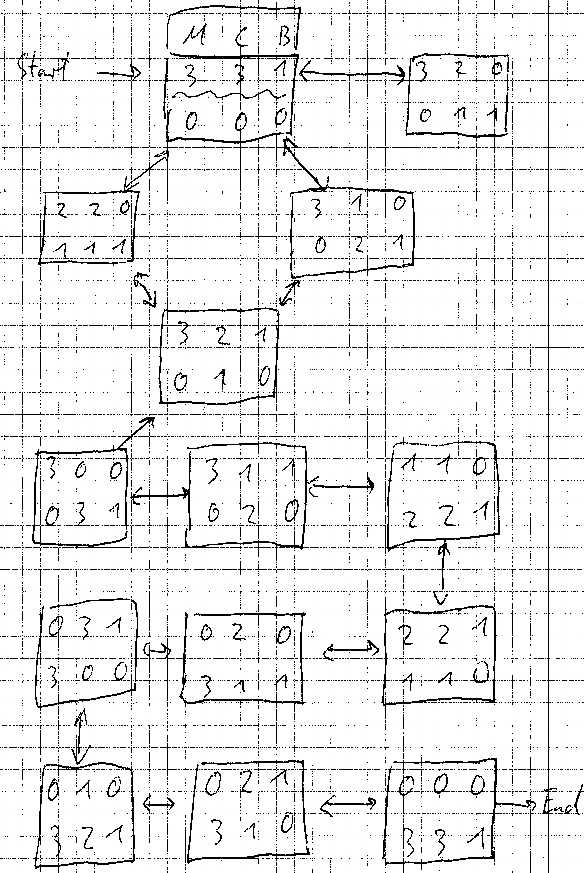
\includegraphics[width=.65\linewidth]{missionaries_cropped.jpg}
 \caption{The state space graph of the missionary-cannibal-boat problem. The columns denote the objects (M, C, B), the rows the location (side of the river). It turns out that most possible states are not allowed by the problem statement.}
\end{figure}

\begin{figure}[ht]
 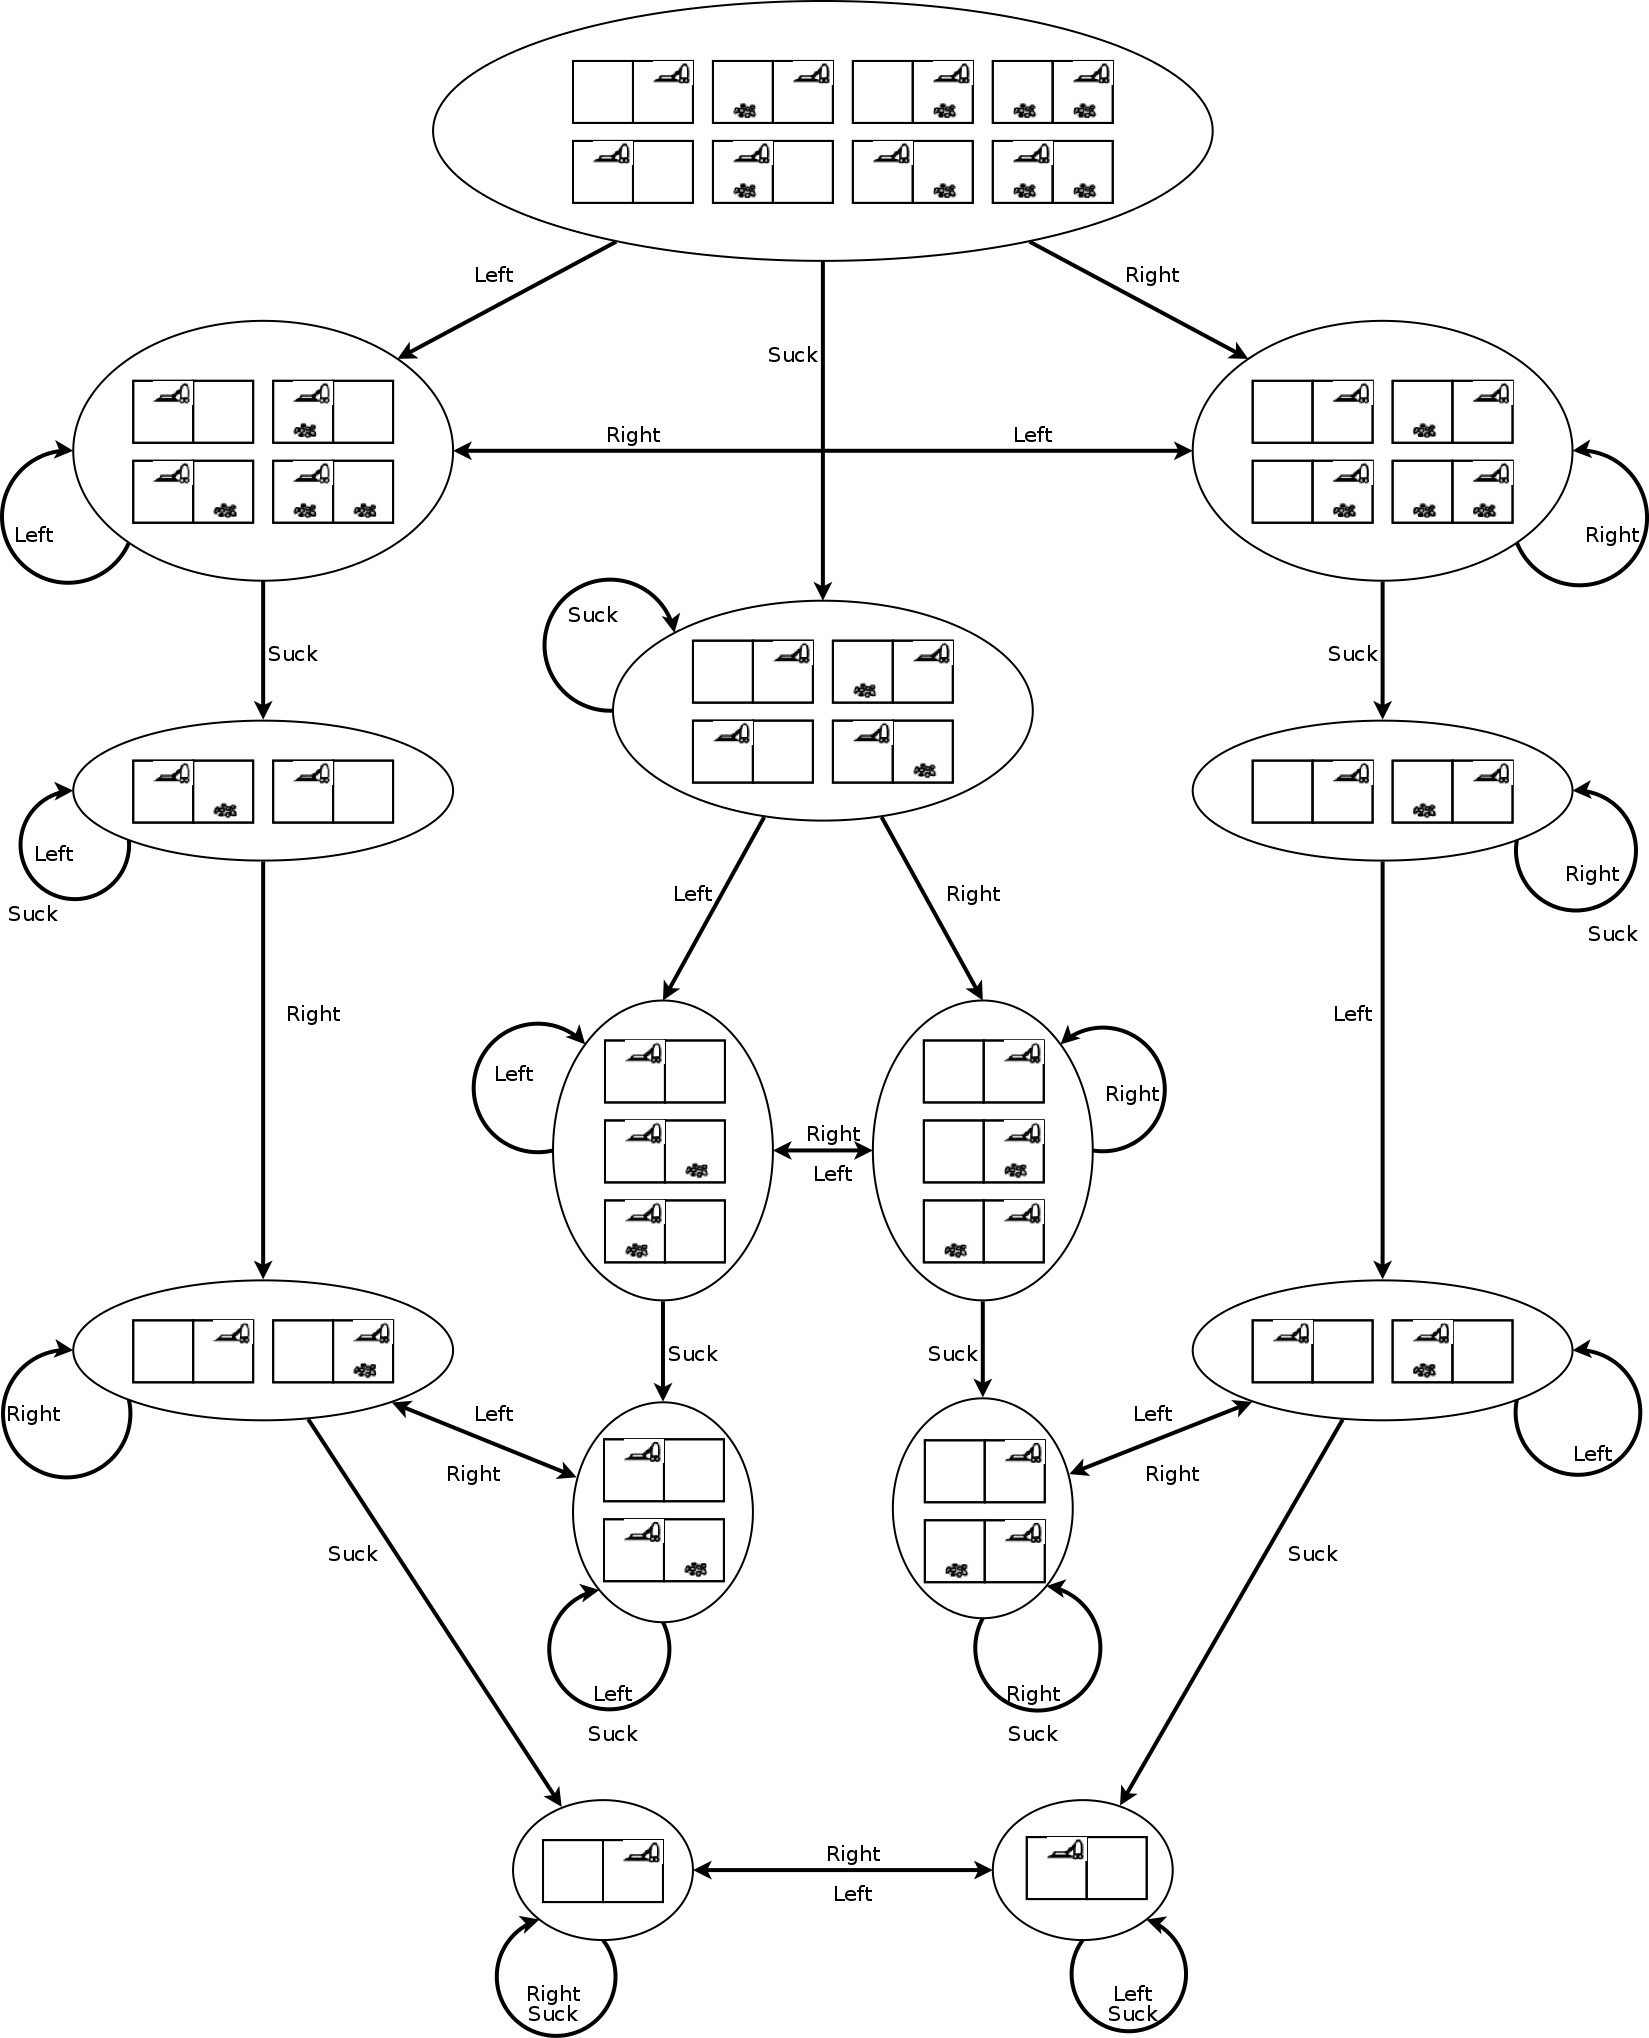
\includegraphics[width=.99\linewidth]{roomba.png}
 \caption{The state space of 'vaccuum world without sensors'. }
\end{figure}

%\newpage
%\appendix
%\lstinputlisting[language=python]{ia_05_01.py}
%\newpage
%\lstinputlisting[language=python]{ia_05_02.py}
\end{document}